\begin{frame}[shrink]
  \frametitle{Agenda}
  \begin{itemize}
    \item Introducción:
      \begin{itemize}
        \item Aplicaciones web y la seguridad.
        \item Qué es un Web Application Firewall (WAF).
        \item Comunicaciones cifradas. Transport Layer Security (TLS).
      \end{itemize}
    \item Situación actual. Estado del arte:
      \begin{itemize}
        \item Soluciones WAF privativas.
        \item Soluciones WAF de software libre.
        \item Uso de HTTP / HTTPS.
      \end{itemize}
    \item Solución.
      \begin{itemize}
        \item Objetivo.
        \item Diseño.
        \item Arquitectura.
      \end{itemize}
    \item Conclusiones.
    \item Test y resultados.
  \end{itemize}
\end{frame}

\section{Introducción}
\subsection{Aplicaciones web y la seguridad}
\begin{frame}[shrink]
  \frametitle{Aplicaciones web y la seguridad}
  \begin{block}{Premisa}
     La seguridad 100\% no existe.
  \end{block}
  Las aplicaciones web están siendo atacadas continuamente.
  \begin{figure}
    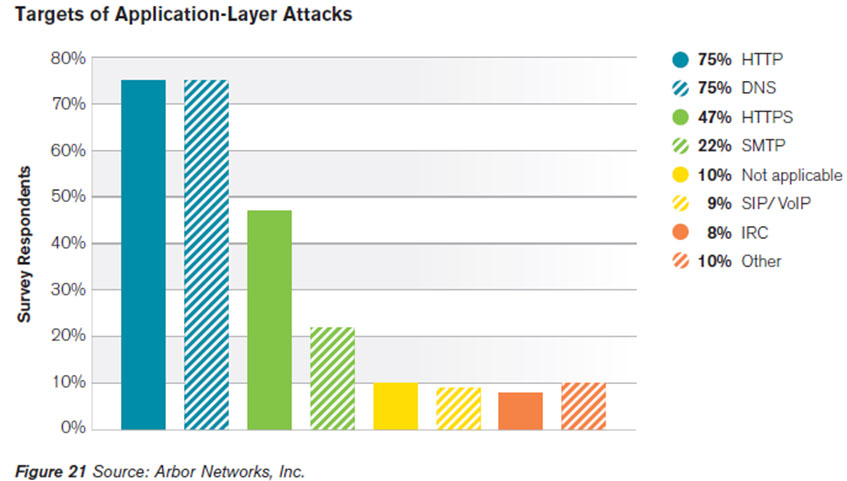
\includegraphics[width=0.35\textwidth]{fig/application-attacks-2}%
    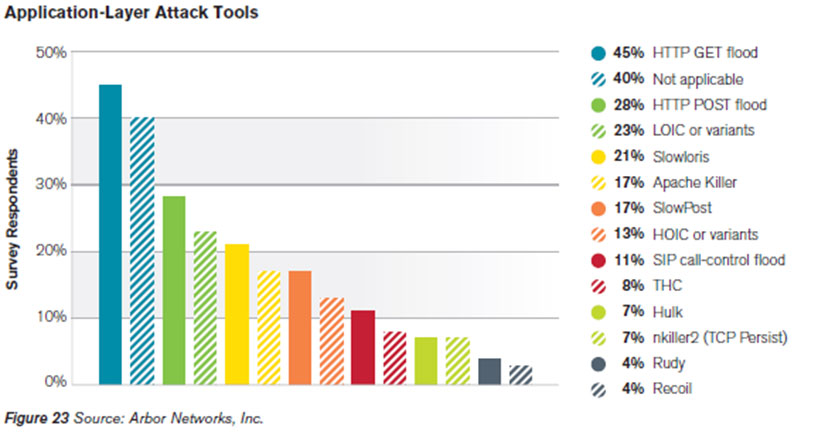
\includegraphics[width=0.35\textwidth]{fig/application-attacks-1}
    \label{fig:applicationattacks}
    \caption{Ataques en capa de aplicación (fuente Arbor~\cite{articleArbor})}
  \end{figure}
  \begin{block}{Conclusión}
    Se debe realizar un esfuerzo continuo para mejor la seguridad de las plataformas web.
  \end{block}
\end{frame}


\begin{frame}[shrink]
  \frametitle{Vulnerabilidades y evolución de los canales cifrados}
  En los últimos años se ha descubierto múltiples vulnerabilidades críticas en los canales TLS.
  \begin{center}
    \rowcolors[]{1}{blue!20}{blue!5}
    \begin{tabular}{|l|l|}
      \hline
      {\bf Vulnerabilidad}   			& {\bf Componente afectado}\\
      \hline
      POODLE											&   SSL ver. 3.0        \\
      \hline
      BEAST												&   TLS ver. 1.0        \\
      \hline
      CRIME                       &   TLS compression     \\
      \hline
      BREACH                      &   HTTP compression    \\
      \hline
      Heartbleed                  &   OpenSSL ver. 1.0.1  \\
      \hline
    \end{tabular}
  \end{center}
  \begin{block}{Conclusión}
    La solución, en la mayoría de de los casos, consiste en desactivar las versiones o el componente afectados y el riesgo de afectar la funcionalidad de la plataforma es bajo (dependiendo del entorno).
  \end{block}
\end{frame}


\begin{frame}[shrink]
  \frametitle{Uso de canales cifrados}
  El uso de 
\end{frame}
